\documentclass[oneside,final,14pt,a4paper]{extreport}

\usepackage{tempora} % Times New Roman alike font

\usepackage{vmargin}
\setpapersize{A4}
\setmarginsrb{2.5cm}{2.2cm}{2.2cm}{2.2cm}{0pt}{10mm}{0pt}{13mm}
\usepackage{setspace}
\setstretch{1.5}
\usepackage{indentfirst}
\parindent=1.25cm

%%%%% ADDED TO SUPPORT TT BOLD FACES %%%%
\DeclareFontShape{OT1}{cmtt}{bx}{n}{<5><6><7><8><9><10><10.95><12><14.4><17.28><20.74><24.88>cmttb10}{}
\renewcommand{\ttdefault}{pcr}
%%%%% END %%%%%%%%%%%%%%%%%%%%%%%%%%%%%%%

\usepackage{atbegshi,picture}
\usepackage[T1,T2A]{fontenc}
\usepackage[utf8]{inputenc}

\usepackage[english]{babel}
\usepackage[backend=biber,style=ieee,autocite=inline]{biblatex}
\addbibresource{./bibliography.bib}
\DefineBibliographyStrings{english}{
  bibliography = {References},
}
\usepackage{blindtext}

\usepackage{pdfpages}
\newenvironment{bottompar}{\par\vspace*{\fill}}{\clearpage}
\usepackage{amsmath,amsfonts}
\usepackage{url}
\usepackage{amsthm}
\newtheorem{theorem}{Theorem}
\newtheorem{corollary}{Corollary}
\newtheorem{lemma}{Lemma}
\newtheorem{proposition}{Proposition}
\theoremstyle{definition}
\newtheorem{definition}{Definition}
\theoremstyle{remark}
\newtheorem*{remark}{Remark}
\theoremstyle{remark}
\newtheorem*{example}{Example}

\usepackage{float}
\usepackage{graphicx}
\graphicspath{{figs/}} %path to images
\usepackage{array}
\usepackage{multirow,array}
\usepackage{caption}
\usepackage{subcaption}
\usepackage{hyperref}
\hypersetup{colorlinks=true, linkcolor=black, citecolor=black}
\usepackage{paralist}
\usepackage{listings}
\usepackage{zed-csp}
\usepackage{fancyhdr}
\usepackage{csquotes}
\usepackage{color}
% \usepackage{anyfontsize}
% \usepackage{mathptmx}
% \usepackage{t1enc}

\usepackage{chngcntr}
\usepackage{upgreek}
\usepackage{bm}
\usepackage{hyperref}
\usepackage{booktabs}
\usepackage{multirow}
\usepackage{longtable}
\usepackage[font=singlespacing, labelfont=bf]{caption}
%Hints
\newcommand\pic[1]{(Fig. \ref{#1})} %Ref on figure
\newcommand\tab[1]{(Tab. \ref{#1})} %Ref on table

\setlength{\headheight}{32.0976pt}
\usepackage{enumitem}
\newlist{inlinelist}{enumerate*}{1}
\setlist*[inlinelist,1]{%
  label=(\arabic*),
}

% \setcounter{secnumdepth}{4}
\captionsetup[table]{labelfont={normalfont}, name={TABLE}, labelsep={newline}}
\setlength{\parindent}{2em}
\DeclareCaptionLabelSeparator{figSep}{.\quad}
\captionsetup[figure]{labelfont={normalfont}, name={Fig.}, labelsep=period}
\counterwithin{figure}{chapter}

% \usepackage{titlesec}
% \titleformat{\section}[hang]{\fontsize{20}{24}\selectfont\filcenter}{\Roman{section}}{1em}{}
% \titleformat{\subsection}[hang]{\itshape}{\Alph{subsection}.}{1em}{}[]
% \titleformat{\subsubsection}[runin]{\itshape}{\arabic{subsubsection})}{1em}{}[$:$]
% \titlespacing{\subsubsection}{1em}{1em}{1em}
% \titleformat{\paragraph}[runin]{\itshape}{\alph{paragraph})}{1em}{}[$:$\quad]
% \titlespacing{\paragraph}{2em}{1em}{1em}

\usepackage{placeins} % for \FloatBarrier

\pagestyle{fancyplain}

% remember section title
\renewcommand{\chaptermark}[1]%
	{\markboth{\chaptername~\thechapter~--~#1}{}}

% subsection number and title
\renewcommand{\sectionmark}[1]%
	{\markright{\thesection\ #1}}

\rhead[\fancyplain{}{\bf\leftmark}]%
      {\fancyplain{}{\bf\thepage}}
\lhead[\fancyplain{}{\bf\thepage}]%
      {\fancyplain{}{\bf\rightmark}}
\cfoot{} %bfseries


\newcommand{\dedication}[1]
   {\thispagestyle{empty}

   \begin{flushleft}\raggedleft #1\end{flushleft}
}

\newcommand{\reformulate}[1]{\textcolor{red}{\textbf{#1}}}


\begin{document}

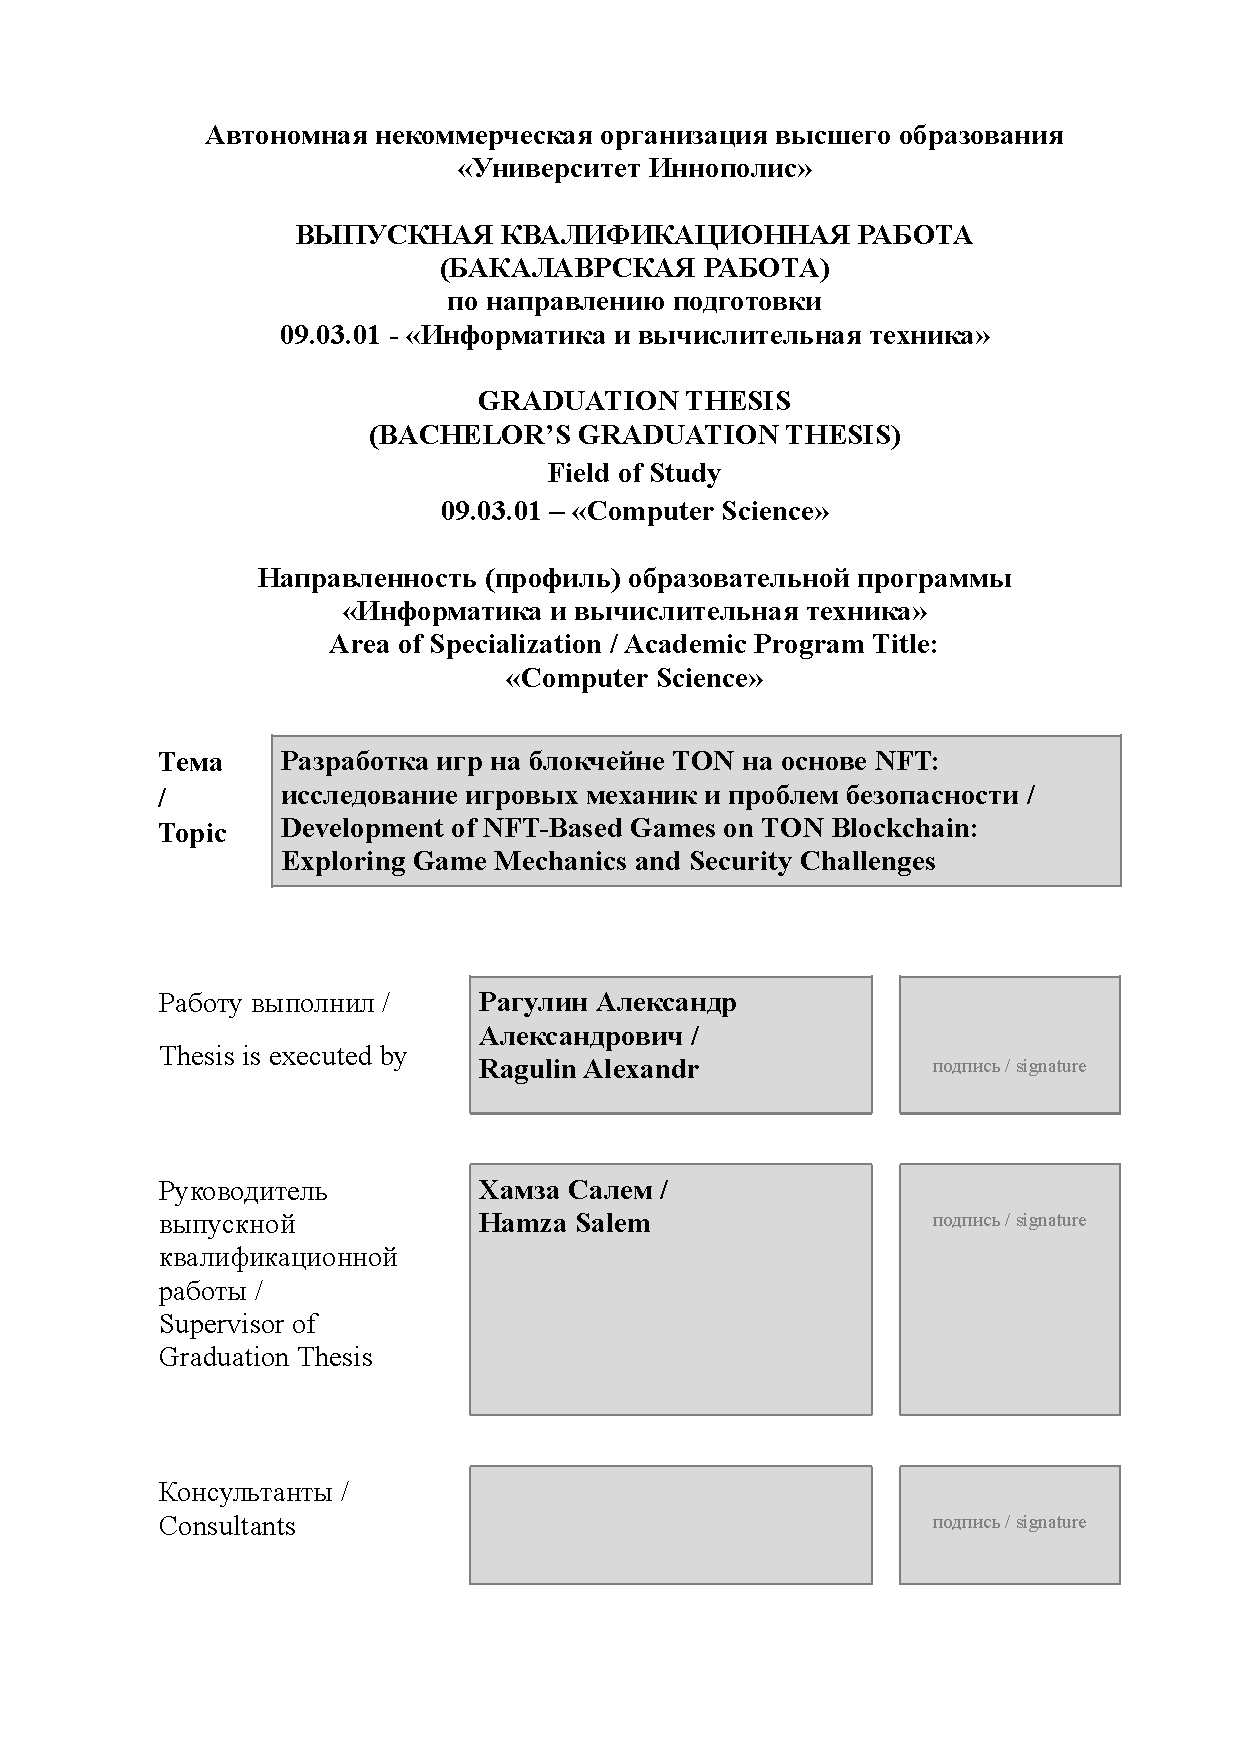
\includepdf[pages=-,offset=2cm -3cm]{title.pdf}
\tableofcontents
\listoftables
\listoffigures
\newpage


% TODO: uncomment
\begin{abstract}
% skip one line to make the abstract start with indent

% TODO:
% My abstract starts from here.
\end{abstract}

\setcounter{page}{8}
% NOTE:
% set manually the number, from which Chapter 1 starts!
% Why do we put 7 in this case?
% Title page - page 2
% Contents - page 3, page 4
% List of tables - page 5
% List of figures - page 6
% Abstract - page 7
% Chapter 1 - page 8
% In your thesis the counter number can be different, please count carefully and insert the corresponding number.

\chapter{Introduction}
% \label{chap:intro}
% \chaptermark{Optional running chapter heading}
% \section{Spacing \& Type}
% \label{sec:section}


The rise of NFT-based games has introduced a paradigm shift in game mechanics,
particularly in digital asset ownership and player-driven economies
\cite{min_blockchain_2019}. However, despite the potential for innovation, there
is noticeable stagnation in the development of novel game mechanics. Most
existing games replicate established patterns, limiting the scope for deeper
engagement and unique gameplay experiences \cite{jiang_cryptokitties_2021}. This
gap highlights the need for new approaches to revitalize the blockchain gaming
landscape.

Emerging blockchain technologies, specifically the TON (The Open Network)
blockchain, present a unique opportunity to address this challenge. TON’s
architecture, designed for infinite scalability and advanced sharding,
introduces a highly decentralized and resilient network. These features enhance
transaction efficiency and enable developers to implement mechanics that were
previously unfeasible on platforms like Ethereum due to scalability constraints
and high transaction costs.
Additionally, TON’s smart contract technology, while similar in purpose to
Ethereum’s, offers significant structural and executional advantages, enabling
more versatile game interactions\cite{durov_telegram_nodate}.

This study adopts a three-pronged approach to explore how TON’s distinctive
capabilities can enable innovative game mechanics and provide a path forward for
the stagnating NFT gaming space:
\begin{enumerate}
	\item An overview of TON’s architecture, focusing on its scalability,
	      sharding, and smart contract capabilities.
	\item A literature review of existing and potential game mechanics, with an
	      emphasis on those that leverage blockchain technologies.
	\item A practical demonstration showcasing secure and scalable mechanics
	      enabled by TON’s features, using a prototype or conceptual example.
\end{enumerate}

By bridging the gap in current research, this paper aims to provide both
theoretical insights and practical guidance for leveraging TON in blockchain
gaming. The broader implications of this research include improving user
engagement, fostering novel gameplay experiences, and setting the stage for
sustainable player-driven economies. By combining an analysis of TON’s technical
advantages with concrete examples, this study seeks to inspire developers and
researchers to explore untapped possibilities within this dynamic and evolving
space.

\chapter{Literature Review}
% \label{chap:lr}
% \chaptermark{Second Chapter Heading}

\section{Introduction to Blockchain in Gaming}

Blockchain technology has revolutionized various industries by providing
decentralized, secure, and transparent systems for data management and
transactions. In gaming, blockchain has introduced significant innovations,
particularly through the integration of non-fungible tokens (NFTs) and
decentralized economies\cite{chen_blockchain_2020, bhand_mage_2024}. These technologies have reshaped traditional gaming by
enabling true ownership of in-game assets, allowing players to trade, sell, or
utilize digital items across platforms without relying on centralized control

The concept of player-driven economies, supported by blockchain, has evolved
into a defining feature of NFT-based games. Unlike traditional games, where
assets remain locked within closed ecosystems, blockchain-enabled games empower
players to generate real-world value from their in-game efforts. This paradigm
shift has captured the attention of both developers and players, leading to the
rapid growth of NFT-based games over the past decade \cite{bhand_mage_2024}.

Despite their promise, blockchain technologies in gaming face notable
challenges. Early pioneers of the space, such as collectible-focused games and
play-to-earn models, have demonstrated the feasibility of integrating
blockchain.\cite{jiang_cryptokitties_2021} However, these implementations often rely on basic mechanics that
limit gameplay innovation and long-term engagement. This stagnation calls for
further exploration of blockchain’s potential to create deeper, more
interactive, and more dynamic gaming experiences

In this context, blockchain serves as both a technological enabler and a
creative challenge. By examining the trajectory of blockchain in gaming, this
review seeks to contextualize its evolution, highlight its current applications,
and set the stage for exploring advanced blockchain platforms, such as The Open
Network (TON), that may redefine the boundaries of game design and player
interaction \cite{stamatakis_blockchain-powered_2024}.


\section{Existing NFT-Based Games and Mechanics}

NFT-based games have emerged as a transformative force in the gaming industry,
leveraging blockchain technology to create unique digital assets that players
can own, trade, and monetize \cite{shetty_serverfi_2024}. These games typically center
around mechanics such as asset collection, trading, and play-to-earn models,
which capitalize on the immutable and transparent nature of blockchain
\cite{pfeiffer_blockchain_2020, stamatakis_blockchain-powered_2024}

One of the earliest and most influential examples is the use of collectible
NFTs, where players acquire and trade digital assets that are provably rare and
unique. These mechanics were popularized by games that revolved around
ownership and scarcity, often appealing to collectors and
investors\cite{shetty_serverfi_2024}. Another prevalent mechanism is breeding,
which allows players to combine assets to produce new, unique NFTs, a feature
that adds an element of creativity and strategy to gameplay
\cite{pfeiffer_blockchain_2020, jiang_cryptokitties_2021}.

Play-to-earn models have further evolved the blockchain gaming space by offering
players tangible rewards for their time and skills. These systems enable users
to generate cryptocurrencies or other blockchain-based tokens through in-game
activities, effectively turning games into economic ecosystems \cite{shetty_serverfi_2024}.
The promise of financial incentives has attracted millions of players worldwide,
but it has also introduced sustainability challenges, as many play-to-earn games
rely on speculative market dynamics \cite{stamatakis_blockchain-powered_2024}.

Despite their innovation, these mechanics have shown clear limitations. Many
existing NFT games focus narrowly on economic interactions, often at the expense
of engaging gameplay. This overemphasis on financial incentives has led to
repetitive and shallow mechanics, failing to fully leverage blockchain's
potential to create dynamic, interactive, and immersive experiences \cite{stamatakis_blockchain-powered_2024}

As the field matures, it is becoming evident that the current reliance on
established patterns—such as trading, collecting, and play-to-earn—limits the
scope of NFT-based gaming. To move beyond these constraints, developers must
explore new mechanics and game designs that incorporate blockchain as a
foundational tool for interaction and innovation, rather than just a financial
mechanism \cite{shetty_serverfi_2024}. This necessity sets the stage for examining advanced
blockchain solutions like TON, which offer the technical capabilities to break
free from these traditional molds.

\section{Challenges in Current Blockchain Gaming Ecosystems}

While blockchain technology has introduced innovative possibilities for gaming,
it also presents significant challenges that limit its broader adoption and the
development of engaging gameplay experiences. These challenges span technical,
economic, and design-related aspects, collectively hindering the evolution of
blockchain gaming.

\subsection{Technical Challenges}

Scalability remains one of the most pressing issues in blockchain gaming.
Popular platforms such as Ethereum have struggled to handle the high transaction
volumes generated by successful games, leading to network congestion and
exorbitant gas fees\cite{min_blockchain_2019}. This creates a barrier for both developers, who must
navigate these limitations to implement mechanics, and players, who face high
costs for basic interactions.

Interoperability is another critical obstacle. Most blockchain games operate
within isolated ecosystems, making it difficult for assets and currencies to be
transferred across different games or platforms. This fragmentation reduces the
value of blockchain’s promise of open, decentralized ecosystems, limiting its
appeal to mainstream developers and players\cite{jiang_cryptokitties_2021}.

\subsection{Economic Challenges}

The heavy reliance on play-to-earn models has introduced significant economic
risks. These models often create economies driven by speculation, where asset
values depend on continued user growth. Such systems are prone to instability,
leading to unsustainable boom-and-bust cycles that undermine long-term player
trust and engagement\cite{jiang_cryptokitties_2021, jiang_towards_2022}.
Additionally, the focus on financial incentives can overshadow gameplay quality,
reducing the appeal of games as entertainment.

\subsection{Game Design Challenges}

Designing engaging and innovative gameplay within the constraints of blockchain
technology is a complex task. Many developers default to simplistic mechanics
such as trading and collecting, which, while leveraging blockchain’s strengths,
fail to offer rich, interactive experiences. Furthermore, the technical
complexity of blockchain development poses a steep learning curve for game
designers, limiting the exploration of creative mechanics that take full
advantage of blockchain’s capabilities.

These challenges underscore the need for blockchain solutions that address
scalability, interoperability, and economic sustainability while empowering
developers to innovate. Emerging platforms like TON, with their advanced
architectures and enhanced transaction efficiencies, offer potential pathways to
overcome these barriers and redefine the blockchain gaming landscape.

% \section{Innovation in NFT mechanics}
%
% % tags: Game mechanics
%
% % Innovations (or lack thereof) in NFT gaming mechanics
% % - [ ] Summary of relevant sources.
% % - [ ] How it relates to your research.
% % - [ ] Identified gaps.
%
% The stagnation in the development of innovative gaming mechanics within
% blockchain-based games is largely attributed to persistent challenges in
% maintaining player engagement and market stability. While blockchain technology
% has enabled the introduction of advanced economic models, gameplay mechanics
% often remain insufficiently developed, leading to an overreliance on financial
% incentives rather than fostering engaging gameplay experiences.
%
% Blockchain-based games have pioneered novel economic models, such as those
% outlined in the ServerFi framework, which focus on enhancing player engagement
% through mechanisms like asset synthesis and continuous reward distribution
% \cite{shetty_serverfi_2024}. However, many blockchain games face significant
% challenges in player retention. For instance, a case study on Aavegotchi
% demonstrated that a limited number of dedicated players drive most engagement,
% highlighting the lack of widespread appeal \cite{jiang_towards_2022}.
%
% \reformulate{Technological Limitations}
%
% The inherent complexity of blockchain technology presents a significant obstacle
% for game developers, restricting their ability to explore and implement
% innovative mechanics. While middleware solutions are being developed to simplify
% integration, these technologies remain in their nascent stages
% \cite{shcherba_blockchain_2021}. Furthermore, the prevalence of fraudulent
% activities and market instability erodes trust in blockchain-based games,
% further inhibiting the progression of innovation in this domain
% \cite{pfeiffer_blockchain_2020}
%
%
% \section{Blockchain-based game mechanics}
%
% % tags: Game mechanics
%
% % - [ ] Summary of relevant sources.
% % - [ ] How it relates to your research.
% % - [ ] Identified gaps.
%
%
% \section{Security Challenges}
%
% % Security challenges in blockchain games
% % - [ ] Summary of relevant sources.
% % - [ ] How it relates to your research.
% % - [ ] Identified gaps.
%
% \section{TON's Scalability and Game Applications}
%
% % Tags: Technical, TON
%
%
% % Technical capabilities of TON (e.g., scalability, sharding, smart contracts)
% % - [ ] Summary of relevant sources.
% % - [ ] How it relates to your research.
% % - [ ] Identified gaps.
%
% \section{Comparative Analysis of the TON Blockchain and Other Leading Blockchain Platforms}
%
% % Comparative studies on TON vs. other blockchains (e.g., Ethereum, Solana)
% % - [ ] Summary of relevant sources.
% % - [ ] How it relates to your research.
% % - [ ] Identified gaps.
%
% \section{Conclusion}
%
% % - [ ] Conclusion: Summarize findings,
% % - [ ] justify your focus on TON,
% % - [ ] and outline your methodological approach (e.g., "By leveraging TON's
% %   unique scalability and sharding capabilities, this study addresses the
% %   stagnation of NFT mechanics.").
%
% Despite these challenges, there remains considerable potential for growth in
% the field as developers experiment with alternative models and focus on
% refining gameplay mechanics, indicating that the observed stagnation may only
% be temporary

% TODO: uncomment
% \chapter{Methodology}
% \label{chap:met}

% \chapter{Implementation}
\label{chap:impl}

\ldots
% \chapter{Evaluation and Discussion}
\label{chap:eval}

\ldots
% \chapter{Conclusion}
\label{chap:conclusion}

\ldots

%% REFERENCES
\printbibliography[heading=bibintoc,title={Bibliography cited}]
% \appendix
\chapter{Extra Stuff}
\blindtext

\chapter{Even More Extra Stuff}
\blindtext
\end{document}
